%  LaTeX support: latex@mdpi.com 
%  In case you need support, please attach all files that are necessary for compiling as well as the log file, and specify the details of your LaTeX setup (which operating system and LaTeX version / tools you are using).

% You need to save the "mdpi.cls" and "mdpi.bst" files into the same folder as this template file.

%=================================================================
\documentclass[journal,article,submit,moreauthors,pdftex,10pt,a4paper]{mdpi} 

%
%--------------------
% Class Options:
%--------------------
% journal
%----------
% Choose between the following MDPI journals:
% actuators, admsci, aerospace, agriculture, agronomy, algorithms, animals, antibiotics, antibodies, antioxidants, applsci, arts, atmosphere, atoms, axioms, batteries, behavsci, beverages, bioengineering, biology, biomedicines, biomimetics, biomolecules, biosensors, brainsci, buildings, carbon, cancers, catalysts, cells, challenges, chemosensors, children, chromatography, climate, coatings, computation, computers, condensedmatter, cosmetics, cryptography, crystals, data, dentistry, designs, diagnostics, diseases, diversity, econometrics, economies, education, electronics, energies, entropy, environments, epigenomes, fermentation, fibers, fishes, fluids, foods, forests, futureinternet, galaxies, games, gels, genealogy, genes, geosciences, geriatrics, healthcare, horticulturae, humanities, hydrology, informatics, information, infrastructures, inorganics, insects, instruments, ijerph, ijfs, ijms, ijgi, ijtpp, inventions, jcdd, jcm, jdb, jfb, jfmk, jimaging, jof, jintelligence, jlpea, jmse, jpm, jrfm, jsan, land, languages, laws, life, literature, lubricants, machines, magnetochemistry, marinedrugs, materials, mathematics, mca, mti, medsci, medicines, membranes, metabolites, metals, microarrays, micromachines, microorganisms, minerals, molbank, molecules, mps, nanomaterials, ncrna, neonatalscreening, nutrients, particles, pathogens, pharmaceuticals, pharmaceutics, pharmacy, philosophies, photonics, plants, polymers, processes, proteomes, publications, recycling, religions, remotesensing, resources, risks, robotics, safety, scipharm, sensors, separations, sexes, sinusitis, socsci, societies, soils, sports, standards, sustainability, symmetry, systems, technologies, toxics, toxins, tropicalmed, universe, urbansci, vaccines, vetsci, viruses, vision, water
%---------
% article
%---------
% The default type of manuscript is article, but can be replaced by: 
% addendum, article, book, bookreview, briefreport, casereport, changes, comment, commentary, communication, conceptpaper, correction, conferenceproceedings, conferencereport, expressionofconcern, meetingreport, creative, datadescriptor, discussion, editorial, essay, erratum, hypothesis, interestingimage, letter, newbookreceived, opinion, obituary, projectreport, reply, retraction, review, perspective, preprints, shortnote, supfile, technicalnote, viewpoint
% supfile = supplementary materials
%----------
% submit
%----------
% The class option "submit" will be changed to "accept" by the Editorial Office when the paper is accepted. This will only make changes to the frontpage (e.g. the logo of the journal will get visible), the headings, and the copyright information. Also, line numbering will be removed. Journal info and pagination for accepted papers will also be assigned by the Editorial Office.
%------------------
% moreauthors
%------------------
% If there is only one author the class option oneauthor should be used. Otherwise use the class option moreauthors.
%---------
% pdftex
%---------
% The option pdftex is for use with pdfLaTeX. If eps figure are used, remove the option pdftex and use LaTeX and dvi2pdf.

%=================================================================
\firstpage{1} 
\makeatletter 
\setcounter{page}{\@firstpage} 
\makeatother 
\articlenumber{x}
\doinum{10.3390/------}
\pubvolume{xx}
\pubyear{2016}
\copyrightyear{2016}
\externaleditor{Academic Editor: name}
\history{Received: date; Accepted: date; Published: date}

%------------------------------------------------------------------
% The following line should be uncommented if the LaTeX file is uploaded to arXiv.org
%\pdfoutput=1

%=================================================================
% Add packages and commands here. The following packages are loaded in our class file: fontenc, calc, indentfirst, fancyhdr, graphicx, lastpage, ifthen, lineno, float, amsmath, setspace, enumitem, mathpazo, booktabs, titlesec, etoolbox, amsthm, hyphenat, natbib, hyperref, footmisc, geometry, caption, url, mdframed

%=================================================================
%% Please use the following mathematics environments: Theorem, Lemma, Corollary, Proposition, Characterization, Property, Problem, Example, ExamplesandDefinitions, Remark, Definition
%% For proofs, please use the proof environment (the amsthm package is loaded by the MDPI class).

%=================================================================
% Full title of the paper (Capitalized)
\Title{Vulnerability of JWT}

% If this is an expanded version of a conference paper, please cite it here: enter the full citation of your conference paper, and add $^\dagger$ in the end of the title of this article.
%\conference{}

% Authors, for the paper (add full first names)
\Author{JUNHWI KIM $^{1,\ddagger}$, BYEONGHYEON YOU $^{1,\ddagger}$ and SANGYOON LEE $^{1,\ddagger}$*}
% Authors, for metadata in PDF
\AuthorNames{Firstname Lastname, Firstname Lastname and Firstname Lastname}

% Affiliations / Addresses (Add [1] after \address if there is only one affiliation.)
\address{%
$^{1}$ \quad School of Computing, Korea Advanced Institute of Science and Technology (KAIST),
Daehak-ro 291, Yuseong-gu, Daejeon 34141, Korea; junhwi.kim23@kaist.ac.kr; byou@kaist.ac.kr; pinetree408@gmail.com}
%$^{2}$ \quad Affiliation 2; e-mail@e-mail.com}

% Contact information of the corresponding author
\corres{Correspondence: pinetree408@gmail.com; Tel.: +82-10-5657-8281}

% Current address and/or shared authorship
%\firstnote{Current address: Affiliation 3} 
%\secondnote{These authors contributed equally to this work.}

% Simple summary
%\simplesumm{}

% Abstract (Do not use inserted blank lines, i.e. \\) 
\abstract{
% TODO
}
%A single paragraph of about 200 words maximum. For research articles, abstracts should give a pertinent overview of the work. We strongly encourage authors to use the following style of structured abstracts, but without headings: 1) Background: Place the question addressed in a broad context and highlight the purpose of the study; 2) Methods: Describe briefly the main methods or treatments applied; 3) Results: Summarize the article's main findings; and 4) Conclusion: Indicate the main conclusions or interpretations. The abstract should be an objective representation of the article, it must not contain results which are not presented and substantiated in the main text and should not exaggerate the main conclusions.}

% Keywords
\keyword{Web session authentication; HTTP cookies; Authentication; } %(list three to ten pertinent keywords specific to the article, yet reasonably common within the subject discipline.)}

% The fields PACS, MSC, and JEL may be left empty or commented out if not applicable
%\PACS{J0101}
%\MSC{}
%\JEL{}

%%%%%%%%%%%%%%%%%%%%%%%%%%%%%%%%%%%%%%%%%%
% Only for the journal Data:

%\dataset{DOI number or link to the deposited data set in cases where the data set is published or set to be published separately. If the data set is submitted and will be published as a supplement to this paper in the journal Data, this field will be filled by the editors of the journal. In this case, please make sure to submit the data set as a supplement when entering your manuscript into our manuscript editorial system.}

%\datasetlicense{license under which the data set is made available (CC0, CC-BY, CC-BY-SA, CC-BY-NC, etc.)}

%%%%%%%%%%%%%%%%%%%%%%%%%%%%%%%%%%%%%%%%%%
% For Conference Proceedings Papers: add the conference title here
%\conferencetitle{}

%\setcounter{secnumdepth}{4}
%%%%%%%%%%%%%%%%%%%%%%%%%%%%%%%%%%%%%%%%%%
\begin{document}

%%%%%%%%%%%%%%%%%%%%%%%%%%%%%%%%%%%%%%%%%%
%% Only for the journal Gels: Please place the Experimental Section after the Conclusions

%%%%%%%%%%%%%%%%%%%%%%%%%%%%%%%%%%%%%%%%%%
% \setcounter{section}{-1} %% Remove this when starting to work on the template.
% \section{How to Use this Template}
% The template details the sections that can be used in a manuscript. Note that the order of article sections may differ from the requirements of the journal (e.g. for the positioning of the Materials and Methods section). Please check the instructions for authors page of the journal to verify the correct order. For any questions, please contact the editorial office of the journal or support@mdpi.com. For LaTeX related questions please contact Janine Daum at latex-support@mdpi.com.

\section{Introduction}

The rise of single page applications (SPAs) and demand for multiplatform compatibility lead us to decouple the front-end from the back-end in system architecture. This trend made Token based authentication become popular recently\cite{authentication}. Following is main advantages of token for authentication:
\begin{itemize}[leftmargin=*,labelsep=4mm]
\item	Stateless and scalable servers
\item	Mobile application ready
\item	Pass authentication to other applications
\item	Security
\end{itemize}

We can easily find token based authentication from anywhere. Applications like Facebook, Twitter, GitHub, and other services from big companies are using token based authentication.

\subsection{The conventional method}
Before we examine how token based authentication works and its benefits, we need to look at the traditional way of authentication.
The HTTP protocol is stateless, this means that if we authenticate to application with a username and password, the application won’t remeber who we are on the next request. Therefore, we would have to authenticate again for each request. The traditional way of having our applications remember who we are is to store the user logged in information on the server. This can be done in a few different ways on the session, usually in memory or stored on the disk\cite{authorization}.

\begin{figure}[H]
\centering
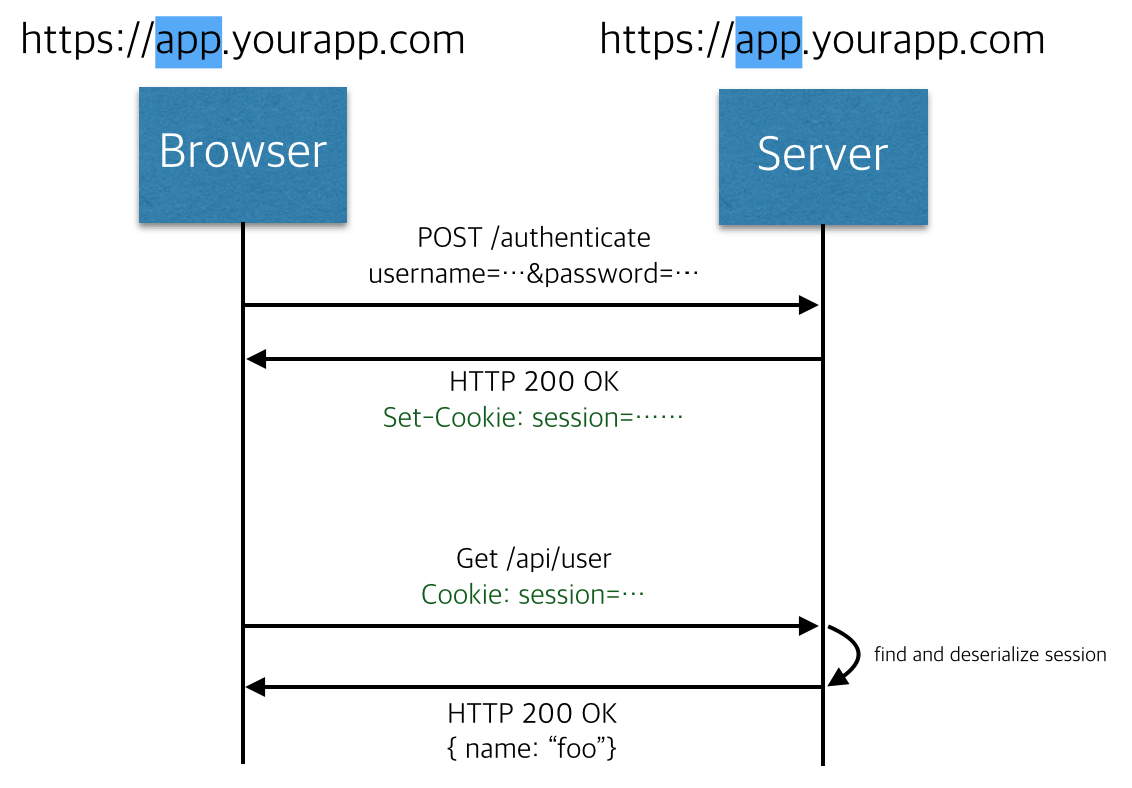
\includegraphics[width=9cm]{figures/traditional}
\caption{This is a figure to explain traditional method. (\textbf{a}) User enters their login credentials. (\textbf{b})Server verifies the credentials are correct and creates a session which is then stored in a database. (\textbf{c}) A cookie with the session ID is placed in the users browser. (\textbf{d}) On subsequent requests, the session ID is verified against the database and if valid the request processed. (\textbf{e}) Once a user logs out of the app, the session is destroyed both client and server side.}
\label{traditional}
\end{figure}

Here is a graph of how a server based authentication workflow would look(Figure~\ref{traditional}). As the web, applications, and the rise of the mobile application have come about, this method of authentication has shown problems\cite{authentication-mobile, attacks}.
The Problems with Server Based Authentication are as follows.
\begin{itemize}[leftmargin=*,labelsep=4mm]
\item	Sessions : Every time a user is authenticated, the server will need to create a record somewhere on our server. This is usually done in memory and when there are many users authenticating, the overhead on your server increases.
\item	Scalability : Since sessions are stored in memory, this provides problems with scalability. As our cloud providers start replicating servers to handle application load, having vital information in session memory will limit our ability to scale.
\item	CORS : As we want to expand our application to let our data be used across multiple mobile devices, we have to worry about cross-origin resource sharing (CORS). When using AJAX calls to grab resources from another domain (mobile to our API server), we could run into problems with forbidden requests.
\item	CSRF : We will also have protection against cross-site request forgery (CSRF). Users are susceptible to CSRF attacks since they can already be authenticated with say a banking site and this could be taken advantage of when visiting other sites.
\end{itemize}

\subsection{The token based method}
Token based authentication is stateless. We are not storing any information about our user on the server or in a session. This concept alone takes care of many of the problems with having to store information on the server\cite{one-time-cookies}.
No session information means your application can scale and add more machines as necessary without worrying about where a user is logged in.
Although this implementation can vary, the gist of it is as follows.
\begin{itemize}[leftmargin=*,labelsep=4mm]
\item User Requests Access with Username / Password
\item Application validates credentials
\item Application provides a signed token to the client
\item Client stores that token and sends it along with every request
\item Server verifies token and responds with data
\end{itemize}

Every single request will require the token. This token should be sent in the HTTP header so that we keep with the idea of stateless HTTP requests. We will also need to set our server to accept requests from all domains using Access-Control-Allow-Origin: *. What’s interesting about designating * in the ACAO header is that it does not allow requests to supply credentials like HTTP authentication, client-side SSL certificates, or cookies.

\begin{figure}[H]
\centering
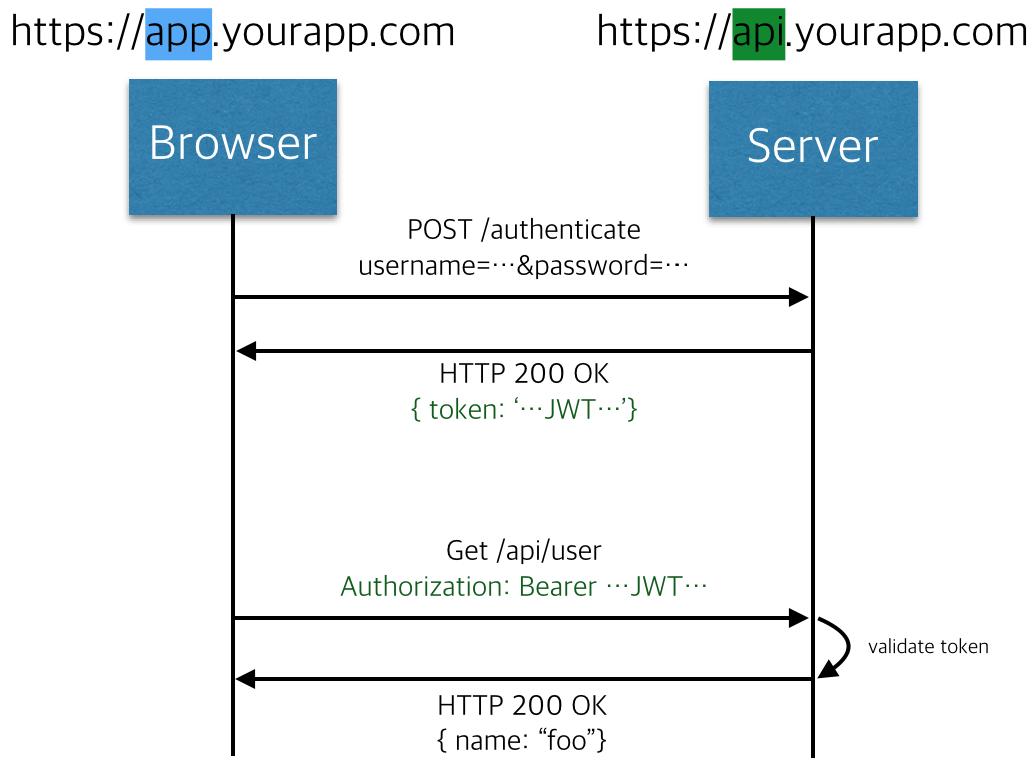
\includegraphics[width=9cm]{figures/tokenbased}
\caption{This is a figure to explain token based method. (\textbf{a}) User enters their login credentials. (\textbf{b}) Server verifies the credentials are correct and returns a signed token. (\textbf{c}) This token is stored client-side, most commonly in local storage - but can be stored in session storage or a cookie as well. (\textbf{d}) Subsequent requests to the server include this token as an additional Authorization header or through one of the other methods mentioned above. (\textbf{e}) The server decodes the token and if the token is valid processes the request. (\textbf{f}) Once a user logs out, the token is destroyed client-side, no interaction with the server is necessary.}
\label{tokenbased}
\end{figure}

Here’s an graph to explain the process(Figure~\ref{tokenbased}). Once we have authenticated with our information and we have our token, we are able to do many things with this token\cite{token-based-fast}.

We could even create a permission based token and pass this along to a third-party application (say a new mobile app we want to use\cite{token-based-mobile}), and they will be able to have access to our data — but only the information that we allowed with that specific token.

\subsection{The Benefits of Token based method}
Tokens stored on client side. Completely stateless, and ready to be scaled. Our load balancers are able to pass a user along to any of our servers since there is no state or session information anywhere. If we were to keep session information on a user that was logged in, this would require us to keep sending that user to the same server that they logged in at. Because it brings problems, some users would be forced to the same server and this could bring about a spot of heavy traffic. Those problems are gone with tokens since the token itself holds the data for that user.

The token, not a cookie, is sent on every request and since there is no cookie being sent, this helps to prevent CSRF attacks. Even if your specific implementation stores the token within a cookie on the client side, the cookie is merely a storage mechanism instead of an authentication one. There is no session based information to manipulate since we don’t have a session. The token also expires after a set amount of time, so a user will be required to login once again. This helps us stay secure. There is also the concept of token revocation that allows us to invalidate a specific token and even a group of tokens based on the same authorization grant\cite{evaluating-authentication}.

Tokens will allow us to build applications that share permissions with another. For example, we have linked random social accounts to our major ones like Facebook or Twitter. When we login to Twitter through a service (let’s say Buffer), we are allowing Buffer to post to our Twitter stream. By using tokens, this is how we provide selective permissions to third-party applications. We could even build our own API and hand out special permission tokens if our users wanted to give access to their data to another application.

We talked a bit about CORS earlier. When our application and service expands, we will need to be providing access to all sorts of devices and applications. Having our API just serve data, we can also make the design choice to serve assets from a CDN. This eliminates the issues that CORS brings up after we set a quick header configuration for our application. Our data and resources are available to requests from any domain now as long as a user has a valid token.

When creating the token, you have a few options. We’ll be diving more into this topic when we secure an API in a follow-up article, but the standard to use would be JSON Web Tokens. This handy debugger and library chart shows the support for JSON Web Tokens. You can see that it has a great amount of support across a variety of languages. This means you could actually switch out your authentication mechanism if you choose to do so in the future.

\subsection{JWT}
%% TODO: 설명

\subsection{vulnerability of JWT}

Tim McLean had reported vulnerabilities of JWT that comes from implementation fault at Auth0 blogs.1 . First vulnerabilities is that token with none signing algorithm bypass the authenticator's validation process. Since anyone can change the JWT token's header, the attacker is able to forge the token's encryption algorithm to none. When attacker makes forged token, token by itself satisfies the JWT format but the token is not what authenticator expected. In order to block this vulnerabilities, the validation method should check if the token's signing method is expected or not. However in 5 official JWT libraries, the token with none signing algorithm could bypass the validation.

Second vulnerabilities is changing the token's signing algorithm from asymmetric to symmetric signing algorithm. In asymmetric signed JWT, public key is used for validation, and private key is used for making the token. When server publish the token with asymmetric signing algorithm, it opens the token and its public key. When the attacker have a token and its public key, he can modify the token claim. Then he alter the signing algorithm to symmetric and sign a key with a public key. The forged token by itself has proper JWT token, but this should not be accepted to server.

We examined 6 official JWT libraries if they had those vulnerabilities, and their patch to vulnerabilites.

Among 6 libraries, 2 libraries were vulnerable to none signing and 3 were vulnerable to altering asymmetric signing to symmetric. To block the none singing vulnerabilities, php-jwt library let server to set the expected algorithm. when the input token's signing algorithm is defer from expected token, then the token is invalid. For the C, libjwt algorithm simply blocks the all none signed token.

For the altiring asymmetric signing to symmetric. Pyjwt set the restriction on HMAC key. If the key as public key format or x509 certificate format, then the key cannot be used as HMAC key. In Node-jsonwebtoken library, when the input token's signing key has public key format, they restrict the token to validated by asymmetric signing method. Finally for the php-jwt, the patch from none singing vulnerabilities also patches this issue.

% The introduction should briefly place the study in a broad context and highlight why it is important. It should define the purpose of the work and its significance. The current state of the research field should be reviewed carefully and key publications cited. Please highlight controversial and diverging hypotheses when necessary. Finally, briefly mention the main aim of the work and highlight the principal conclusions. As far as possible, please keep the introduction comprehensible to scientists outside your particular field of research. Citing a journal paper \cite{ref-journal}. And now citing a book reference \cite{ref-book}.

%%%%%%%%%%%%%%%%%%%%%%%%%%%%%%%%%%%%%%%%%%
\section{Results}
\subsection{Potential vulnerabilities}
We categorized vulnerabilities of JWT into 3 category.
\begin{itemize}[leftmargin=*,labelsep=4mm]
\item Modifiable header
\item Bruteforce attack
\item Replay attack
\end{itemize}

Since JWT header is not encrypted, anyone can modify the header of the JWT which holds the token type and signing algorithm. The two known vulnerabilities were possible because of this modifiable header design of JWT. Bruteforce attack and replay attack will be explained in section *

This section may be divided by subheadings. It should provide a concise and precise description of the experimental results, their interpretation as well as the experimental conclusions that can be drawn.

\subsubsection{Brute force attack}

The important point is JWT is not encrypted and it is just encoded in base64. Therefore, using payload and its signature, you can do brute force attack to exploit the secret used for signature. Since JWT token already contains everything we need to attack, it can be exploited without any communication with server. This means, server doesn't have control over the brute force attack. The dangerous point is secret is not changed frequently and shared in system wide. Therefore, if you success to find the secret even with long time, then you can generate fake token as many times as you want. To prove our idea, we conducted simple bruteforce attack with short secret.data and its hashed value, the verification of the token can be done in local without any limitation, and without any communication with server. It is perfect environment for brute force attack.

Figure~\ref{bruteforce} shows the structure of the token we want to attack. For the attack, we used John the ripper2 brute force tool on i7 CPU, 16GB RAM Ubuntu system. In 3 hours 44 minutes 23 seconds, the tool were able to find the secret key kaistkey.

This experiment shows that brute force attack is really feasible when weak secret key are used. Obviously, long and complex key will make system secure but the point is JWT itself don't have a way to control it. Someone can argue to change the secret periodically, but it will make massive invalidation of issued token and spoil the usability of application.
\begin{figure}[H]
\centering
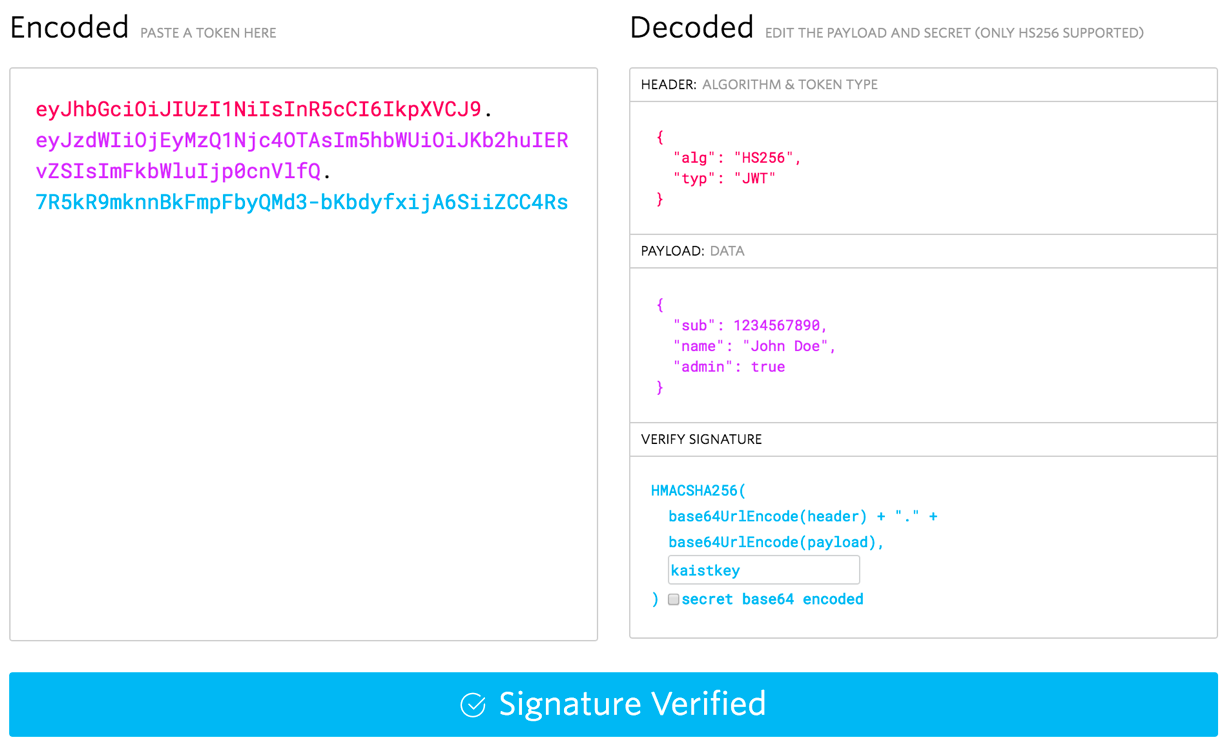
\includegraphics[width=9cm]{figures/bruteforce}
\caption{Simple JWT token to demonstrate brute force attack.}
\label{bruteforce}
\end{figure}

\subsubsection{Replay attack}

In real world, JWT is often used as a authentication session in stateless architecture. In stateless web architecture, server does not store the user state information in its memory. It is client who hold the information. During the communication, client send user status via token claim. User validation solely depends on the input JWT token. The problem is the attacker who stole the token can act like him/her and whenever the attacker tries the replay attack, there is no way to revoke the token in server. Therefore JWT in stateless architecture is always vulnerable to replay attack.

\subsubsection{stateful JWT}

The spread solution to replay attack in JWT authentication session is to use jti claim in JWT. The jti is a unique identifier of a JWT token. which is make the authentication stateful. In stateful JWT, server stores the executed token's jti information in its memory. Whenever server get token with stored jti, server prohibit the replay of the token. Using the jti server can revoke the token and prevent replay attack while losing the advantage of stateless architecture. However, the stateful JWT architecture works similarly as traditional session. Therefore, the stateful JWT is kinds of reinventing the wheel. In fact stateful JWT authentication is more risky than traditional session because there exists implementation fault in JWT libraries because of the immaturity of JWT environment. Therefore there is no reason and advantage to use stateful JWT as an authentication session. In conclusion, JWT in stateless architecture is vulnerable to replay attack and stateful JWT has a potential implementation fault. So we should not use JWT as a persistent authentication token.

%%%%%%%%%%%%%%%%%%%%%%%%%%%%%%%%%%%%%%%%%%
% \subsection{Subsection}

% \subsubsection{Subsubsection}

% Bulleted lists look like this:
% \begin{itemize}[leftmargin=*,labelsep=4mm]
% \item	First bullet
% \item	Second bullet
% \item	Third bullet
% \end{itemize}

% Numbered lists can be added as follows:
% \begin{enumerate}[leftmargin=*,labelsep=3mm]
% \item	First item
% \item	Second item
% \item	Third item
% \end{enumerate}

% The text continues here.

% \subsection{Figures, Tables and Schemes}

% All figures and tables should be cited in the main text as Figure 1, Table 1, etc.

% \begin{figure}[H]
% \centering
% 
\includegraphics[width=3cm]{logo-mdpi}
% \caption{This is a figure, Schemes follow the same formatting. If there are multiple panels, they should be listed as: (\textbf{a}) Description of what is contained in the first panel. (\textbf{b}) Description of what is contained in the second panel. Figures should be placed in the main text near to the first time they are cited. A caption on a single line should be centered.}
% \end{figure}   

% \begin{table}[H]
% \caption{This is a table caption. Tables should be placed in the main text near to the first time they are cited.}
% \centering
%% \tablesize{} %% You can specify the fontsize here, e.g.  \tablesize{\footnotesize}. If commented out \small will be used.
% \begin{tabular}{ccc}
% \toprule
% \textbf{Title 1}	& \textbf{Title 2}	& \textbf{Title 3}\\
% \midrule
% entry 1		& data			& data\\
% entry 2		& data			& data\\
% \bottomrule
% \end{tabular}
% \end{table}

% \subsection{Formatting of Mathematical Components}

% This is an example of an equation:

% \begin{equation}
% \mathbb{S}
% \end{equation}

%% If the documentclass option "submit" is chosen, please insert a blank line before and after any math environment (equation and eqnarray environments). This ensures correct linenumbering. The blank line should be removed when the documentclass option is changed to "accept" because the text following an equation should not be a new paragraph. 
% Please punctuate equations as regular text. Theorem-type environments (including propositions, lemmas, corollaries etc.) can be formatted as follows:
%% Example of a theorem:
% \begin{Theorem}
% Example text of a theorem.
% \end{Theorem}

% The text continues here. Proofs must be formatted as follows:

%% Example of a proof:
% \begin{proof}[Proof of Theorem 1]
% Text of the proof. Note that the phrase `of Theorem 1' is optional if it is clear which theorem is being referred to.
% \end{proof}
% The text continues here.

%%%%%%%%%%%%%%%%%%%%%%%%%%%%%%%%%%%%%%%%%%
\section{Discussion}
\subsection{Proper Usage of JWT}
We recommand to use JWT for one-time authentication between multiple entities in service. One of example is SDK services. In case of SDK services, SDK provider needs to verify the client is authenticated user of service which is using SDK service. Then, client get a signed claim from its service and bring it to SDK provider. If the cryptographic proof, signature, is valid, SDK provider can trust the client and allow to use functions. JWT can be used for this signed claim to prove authentication of client between multiple services.

Another example is stateless micro-service architecture. With the rise of cloud services, many companies are using an Infrastructure as a Service (IaaS), such as Amazon Web Service or Google Cloud Platform and build many small statless components on top of it. For example, if you run stateless file server in your service, authentication server can issue a short-period ticket to download file for authenticated user. Since it has short expiration and is used only once, JWT can be used without weakness that we mentioned above.
% Authors should discuss the results and how they can be interpreted in perspective of previous studies and of the working hypotheses. The findings and their implications should be discussed in the broadest context possible. Future research directions may also be highlighted.

%%%%%%%%%%%%%%%%%%%%%%%%%%%%%%%%%%%%%%%%%%
\section{Materials and Methods}

%Materials and Methods should be described with sufficient details to allow others to replicate and build on published results. Please note that publication of your manuscript implicates that you must make all materials, data, computer code, and protocols associated with the publication available to readers. Please disclose at the submission stage any restrictions on the availability of materials or information. New methods and protocols should be described in detail while well-established methods can be briefly described and appropriately cited.

%Research manuscripts reporting large datasets that are deposited in a publicly available database should specify where the data have been deposited and provide the relevant accession numbers. If the accession numbers have not yet been obtained at the time of submission, please state that they will be provided during review. They must be provided prior to publication.

%Interventionary studies involving animals or humans, and other studies require ethical approval must list the authority that provided approval and the corresponding ethical approval code. 

%%%%%%%%%%%%%%%%%%%%%%%%%%%%%%%%%%%%%%%%%%
\section{Conclusions}
Many examples in web is suggesting use JWT to manage persistent session between server and client. However, it's even worse compared to traditional cookie based session management. As stated in RFC proposal, proper usage of JWT is claiming someone is authenticated from another service in cryptographic reliable way. SDK service or stateless micro service arhitecture is one of example of this kind of usage.
%This section is not mandatory, but can be added to the manuscript if the discussion is unusually long or complex.

%%%%%%%%%%%%%%%%%%%%%%%%%%%%%%%%%%%%%%%%%%
\vspace{6pt} 

%%%%%%%%%%%%%%%%%%%%%%%%%%%%%%%%%%%%%%%%%%
%% optional
%\supplementary{The following are available online at www.mdpi.com/link, Figure S1: title, Table S1: title, Video S1: title.}

%%%%%%%%%%%%%%%%%%%%%%%%%%%%%%%%%%%%%%%%%%
\acknowledgments{This work was supported by Advanced Information Security class(CS548) which was held at KAIST and taught by Kwangjo Kim.}

%%%%%%%%%%%%%%%%%%%%%%%%%%%%%%%%%%%%%%%%%%
\authorcontributions{Junhwi Kim, Byeonghyeon You and Sangyoon Lee performed all parts of the work together.}

%%%%%%%%%%%%%%%%%%%%%%%%%%%%%%%%%%%%%%%%%%
\conflictofinterests{The authors declare no conflict of interest.} 

%%%%%%%%%%%%%%%%%%%%%%%%%%%%%%%%%%%%%%%%%%
%% optional
\abbreviations{The following abbreviations are used in this manuscript:\\

\noindent 
\begin{tabular}{@{}ll}
JWT & JSON Web Tokens
%MDPI & Multidisciplinary Digital Publishing Institute\\
%DOAJ & Directory of open access journals\\
%TLA & Three letter acronym\\
%LD & linear dichroism
\end{tabular}}

%%%%%%%%%%%%%%%%%%%%%%%%%%%%%%%%%%%%%%%%%%
%% optional
%\appendixtitles{no} %Leave argument "no" if all appendix headings stay EMPTY (then no dot is printed after "Appendix A"). If the appendix sections contain a heading then change the argument to "yes".
%\appendixsections{multiple} %Leave argument "multiple" if there are multiple sections. Then a counter is printed ("Appendix A?). If there is only one appendix section then change the argument to ?one? and no counter is printed (?Appendix?).
\appendix
%\section{}
%The appendix is an optional section that can contain details and data supplemental to the main text. For example, explanations of experimental details that would disrupt the flow of the main text, but nonetheless remain crucial to understanding and reproducing the research shown; figures of replicates for experiments of which representative data is shown in the main text can be added here if brief, or as Supplementary data. Mathemtaical proofs of results not central to the paper can be added as an appendix.

%\section{}
%All appendix sections must be cited in the main text. In the appendixes, Figures, Tables, etc. should be labeled starting with `A', e.g., Figure A1, Figure A2, etc. 

%%%%%%%%%%%%%%%%%%%%%%%%%%%%%%%%%%%%%%%%%%
% Citations and References in Supplementary files are permitted provided that they also appear in the reference list here. 
\bibliographystyle{mdpi}

%=====================================
% References, variant A: internal bibliography
%=====================================
\renewcommand\bibname{References}
\begin{thebibliography}{999}
\bibitem{authentication}
Sandhu, R.; Samarati, P. Authentication, access control, and audit. {\em ACM Computing Surveys (CSUR)}, {\bf 1996}, {\em 28(1)}, 241-243.
\bibitem{authorization}
Metz, C. AAA protocols: authentication, authorization, and accounting for the Internet. {\em IEEE Internet Computing}, {\bf 1999}, {\em 3(6)}, 75-79.
\bibitem{authentication-mobile}
Molva, R.; Samfat, D.; Tsudik, G. Authentication of mobile users. {\em IEEE Network} {\bf 1994}, {\em 8(2)}, 26-34.
\bibitem{attacks}
Stoller, S. D. A bound on attacks on authentication protocols. {\em In Foundations of Information Technology in the Era of Network and Mobile Computing} {\bf 2002}, 588-600.
\bibitem{one-time-cookies}
Dacosta, I.; Chakradeo, S.; Ahamad, M.; Traynor, P. One-time cookies: Preventing session hijacking attacks with stateless authentication tokens. {\em ACM Transactions on Internet Technology (TOIT)} {\bf 2012}, {\em 12(1)}, 1.
\bibitem{token-based-fast}
Kbar, G.; Wireless network token-based fast authentication. {\em In Telecommunications (ICT), 2010 IEEE 17th International Conference on IEEE.}, {\bf 2010, April}, 227-233.
\bibitem{token-based-mobile}
Tanvi, P.; Sonal, G.; Kumar, S. M. Token based authentication using mobile phone. {\em In Communication Systems and Network Technologies (CSNT) 2011 International Conference. IEEE.}, {\bf 2011, June}, 85-88.
\bibitem{evaluating-authentication}
Ma, Y.; Feng, J. Evaluating usability of three authentication methods in web-based application. {\em In Software Engineering Research, Management and Applications (SERA), 2011 9th International Conference on  IEEE.}, {\bf 2011}, 81-88.
% Reference 1
%\bibitem{ref-journal}
%Lastname, F.; Author, T. The title of the cited article. {\em Journal Abbreviation} {\bf 2008}, {\em 10}, 142-149.
% Reference 2
%\bibitem{ref-book}
%Lastname, F.F.; Author, T. The title of the cited contribution. In {\em The Book Title}; Editor, F., Meditor, A., Eds.; Publishing House: City, Country, 2007; pp. 32-58.
\end{thebibliography}

%=====================================
% References, variant B: external bibliography
%=====================================
%\bibliography{your_external_BibTeX_file}

%%%%%%%%%%%%%%%%%%%%%%%%%%%%%%%%%%%%%%%%%%
%% optional
%\sampleavailability{Samples of the compounds ...... are available from the authors.}

%%%%%%%%%%%%%%%%%%%%%%%%%%%%%%%%%%%%%%%%%%
\end{document}

